\section{El mercado de los videojuegos}
El videojuego es la industria de ocio y entretenimiento líder tanto en ventas como en crecimiento.

En el año 2015, el mercado del videojuego genero unas ventas de 91.800 millones de dólares, superando el doble de lo producido por la industria cinematográfica (38.300 millones de dólares) y en más de seis veces al mercado de la música (15.000 millones de dólares)~\cite{libro_blanco} según los datos de la Federación Internacional de la Industria Fonográfica.

A continuación, vamos a mostrar con más detalles la información económica del mercado del videojuego, tanto el mundial como el español, así como listar algunas de las tendencias que marcarán el futuro del sector. Los datos de esta sección han sido obtenidos del Libro blanco del desarrollo del videojuego~\cite{libro_blanco}, informe desarrollado por DEV, la asociación española de empresas desarrolladoras de videojuegos.

\subsection{Industria mundial del Videojuego}
El videojuego es actualmente la industria de ocio y entretenimiento líder en ventas y en crecimiento. Superando en dos veces y media la dimensión del mercado del cine y en más de seis veces el de la música, e mercado mundial de los videojuegos generó en 2016 unas ventas de 101.1 millones de dólares. El mercado global del videojuego seguirá creciendo con una tasa anual del 6,6\%, hasta llegar en 2019 a los 118.600 millones de dólares.
\begin{figure}[h]
	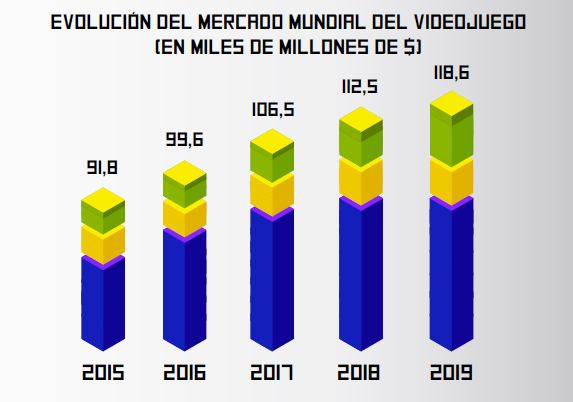
\includegraphics[width=0.8\textwidth]{images/estadodelarte/mercado/crecimiento_mercado_mundial}
	\centering
	\caption{Tabla extraída del Libro Blanco del videojuego (2016)}
\end{figure}

Se estima que, en todo el planeta, haya más de 1.500 millones de jugadores, aunque de entre ellos solo un pequeño 300 millones de usuarios generaría el grueso de las ventas directas, mientras que el resto juegan realizando gastos mucho menos. La mayor parte de los jugadores juegan en plataformas móviles (75\%) y en PC (73\%), siendo las consolas el dispositivo utilizado solamente por el 14\% de los usuarios. Esta diferencia se hace aún más evidente en los países asiáticos y en menor medida en Europa, mientras que en Estados Unidos el uso de las distintas plataformas es más homogéneo.

De entre las distintas plataformas de juegos, segmento con mayor peso en el mercado global en el año 2017 será el mercado de los smartphones, con un ingreso anual de 46.100 millones de dólares, seguido por las consolas de sobremesa, con 33.500 millones de dólares. El segmento Mobile, combinación del segmento de los smartphones con el pequeño segmento de las Tablets, es el que crecerá de forma más contundente, llegando a representar la mitad del total global – unos 64.900 millones de dólares – en 2020.

\begin{figure}[h]
     \centering
     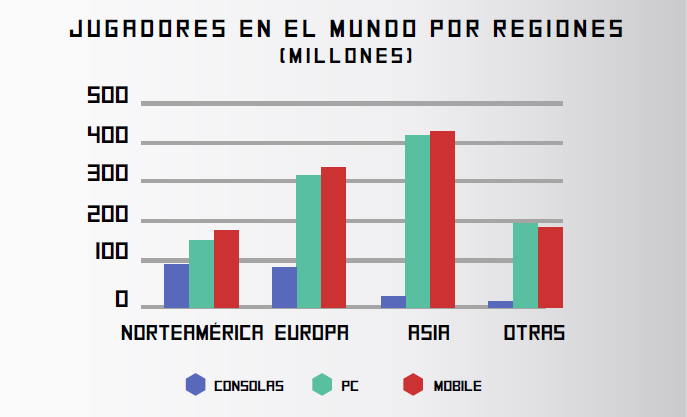
\includegraphics[width=0.8\linewidth]{images/estadodelarte/mercado/jugadores-por-region}
     \caption{Tabla extraída del Libro Blanco del videojuego (2016)}
\end{figure}

Si dividimos el mercado en las distintas regiones geográficas, podemos observar que Asia Pacifico lidera el mercado con un beneficio de 51.200 millones de dólares en el año 2017, un 47\% del total de los ingresos globales. En segunda posición se encuentra el mercado estadounidense que, con 23.500 millones de dólares en 2016, representado prácticamente en su totalidad por Estados Unidos. Más de la mitad de los ingresos de Asia Pacifico son generados en China, con 227.500 millones de dólares. Europa se posiciona con 5 países entre los 10 mayores mercados mundiales por tamaño de ingresos totales: Alemania, Reino Unido, Francia, España e Italia. Sin embargo, la diferencia en tamaño con respecto a los tres primeros mercados (China, Estados Unidos y Japón) es abismal. 

\begin{figure}[h]
	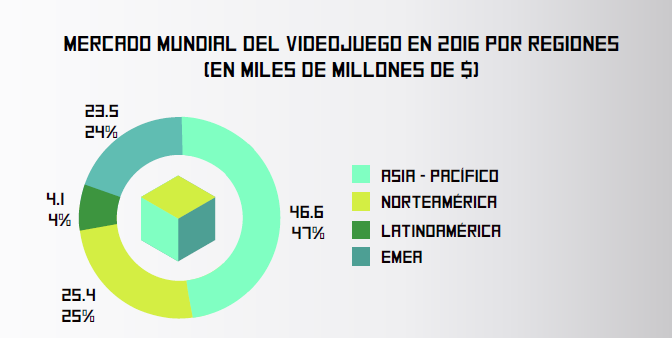
\includegraphics[width=0.8\textwidth]{images/estadodelarte/mercado/ganancia-por-region}
	\centering
	\caption{Tabla extraída del Libro Blanco del videojuego (2016)}
\end{figure}

Por otra parte, los jugadores que realizan un gasto anual más elevado de media son japoneses y surcoreanos, con alrededor de 300\$ de gasto medio, seguidos por los canadienses y estadounidenses (200\$ de gasto medio). China se posiciona entre los países con menor gasto medio por jugador dispuesto a pagar, pero el potencial de crecimiento en términos de poder de adquisición y de número de jugadores es enorme – menos de un tercio de la población juega a videojuegos, frente a una media del 50\% en los demás países occidentales y asiáticos.

Si solo tenemos en cuenta el segmento de los videojuegos para dispositivos móviles, la distribución de las ventas por mercados geográficos permanece casi inalterada con respecto al total. La región Asia-Pacífico representa más de la mitad del mercado Mobile mundial y es liderada por China que mueve 6.500 millones de dólares y crece anualmente del 46,5\%. Las regiones que están experimentando mayor crecimiento son el sureste asiático, con un 69\% anual, Latinoamérica, con un 73\% anual y África-Oriente Medio, con un impresionante 83\%.

\begin{figure}[h]
	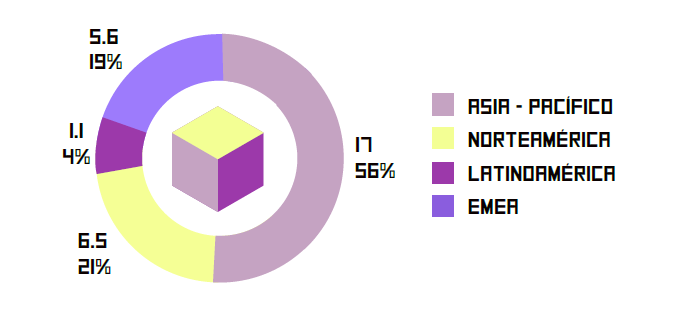
\includegraphics[width=0.8\textwidth]{images/estadodelarte/mercado/ganancia-movil-por-region}
	\centering
	\caption{Mercado mundial, segmento de Dispositivos Móviles (por región)}
\end{figure}

El mercado global de los videojuegos se encuentra muy polarizado, dado que las 25 mayores empresas las que generaron el 67\% de las ganancias globales, sumando un total de 61.600 millones de dólares en 2015. Tencent, que fue la compañía con mayores ingresos en 2015 (8.700 millones de dólares) supera en dos veces el tamaño del mercado en Corea del Sur en su totalidad y en casi 5 veces el español. Por otro lado, las consolidaciones en el sector (como las recientes compras de King por Activision-Blizzard\cite{compra_king} y la de Supercell por Tencent\cite{compra_supercell}) están contribuyendo a aumentar el peso de los gigantes del sector.

\subsection{La industria de los videojuegos en España}
En nuestro país, la industria del videojuego mantiene un ritmo de crecimiento alto, habiéndose incrementado en un 20\% en el último año a pesar de la pasada crisis económica. Actualmente, el sector cuenta con un total de 480 empresas en activo, a las que debemos añadir las 125 iniciativas y proyectos empresariales, que se encuentran a la espera de consolidarse como empresas en el corto o medio plazo.

\begin{figure}[h]
    \centering
    \includegraphics[width=0.8\textwidth]{images/estadodelarte/mercado/crecimiento-españa}
    \caption{Tabla extraída del Libro Blanco del videojuego (2016)}
\end{figure}

Este crecimiento ha sido muy acelerado en el último decenio. De las empresas actuales, el 85\% se fundaron hace menos de 10 años, y el 63\% tienen menos de 5 años. El periodo de crecimiento coincide con la explosión del mercado de los videojuegos para dispositivos móviles a nivel mundial y, en menor medida, la aparición de servicios de distribución digital, como Steam. Estos nuevos mercados fomentaron la aparición de pequeños estudios independientes de plantilla reducida.

Los principales centros de actividad del país son las Comunidades de Madrid y Cataluña, donde se concentra la mitad de los estudios de videojuegos nacionales. A las dos primeras comunidades les sigue la Comunidad Valenciana, que cuenta con un 11\% de las empresas del sector, Andalucía, con un 9\% y el País Vasco, con un 7\%.

\begin{figure}[h]
    \centering
    \includegraphics[width=0.8\textwidth]{images/estadodelarte/mercado/mapa-españa-empresas}
    \caption{En España hay censadas 480 empresas de videojuegos en activo y 125 proyectos empresariales}
\end{figure}

La industria del videojuego en España está formada mayoritariamente por empresas pequeñas, ya que el 95\% de las empresas tiene una plantilla de menos de 50 empleados. Sin embargo, el sector se encuentra muy polarizado: las microempresas (aquellas con menos de 10 empleados), que suponen el 71\% de la masa empresarial, solamente generan el 20\% del empleo nacional, mientras que las medianas y grandes empresas (más de 50 empleados), a pesar de suponer solo el 8\% del total, emplean a casi la mitad (48\%) de los profesionales del sector.

La industria del videojuego es una de las más creativas y se caracteriza por la creación de nueva propiedad intelectual. La mayor parte de las empresas se dedica al desarrollo de IP propia o desarrollo para terceros. Es relevante destacar que muchas empresas se dedican a múltiples actividades, es decir, compaginan el desarrollo de IP propia con el desarrollo para terceros y la formación. Con respecto a 2015, se ha detectado un ligero descenso de estudios que desarrollan IP propia (de 82\% a 76\%).

\begin{figure}[h]
    \centering
    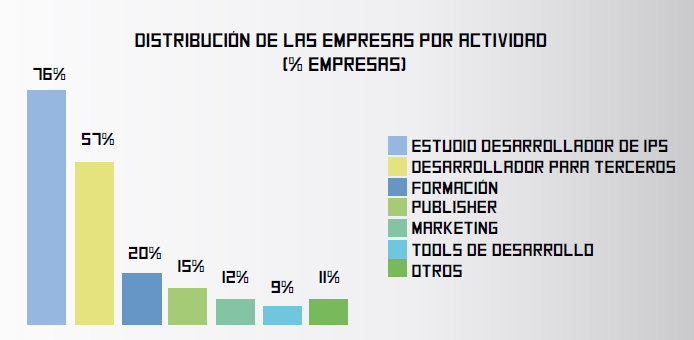
\includegraphics[width=0.8\textwidth]{images/estadodelarte/mercado/desarrollo-ip}
    \caption{Tabla extraída del Libro Blanco del videojuego (2016)}
\end{figure}

La facturación de la industria de desarrollo de videojuegos en España alcanzó los 510,7 millones de euros en 2015, un 24\% más que en el año anterior. El 84\% de la facturación se reparte en igual medida entre los dos grandes polos empresariales de este sector, representados por la Comunidad de Madrid y Cataluña. Les sigue Andalucía que representa un 8\% del total de la facturación nacional. Las sedes de los estudios de más envergadura y, por tanto, de mayor facturación, están localizadas en estas regiones.

Esta tendencia a la polarización también se puede observar en la forma en la que se distribuye la facturación. El 1\% de las empresas concentra el 52\% de la facturación. Las microempresas (facturación menor de 2 millones de euros) representan el 83\% de la masa empresarial, pero solamente el 8\% de la facturación. El 23\% de las empresas españolas, al encontrarse todavía en fases de desarrollo de sus respectivos proyectos, todavía no han iniciado su actividad comercial y, por tanto, no han empezado a facturar.

En cuanto a la procedencia de la facturación, se nota una bajada importante del peso de las ventas de juego en formato físico, cubriendo solo un 6\% de los ingresos. Por otro lado, el 34\% de la facturación proviene de la venta directa digital, mientras que el modelo \"free to play\" representa el 22\%. El casi 40\% restante de la facturación de nuestras empresas proviene de fuentes alternativas, como el desarrollo para terceros, la venta de servicios y la formación. 

Desde un punto de vista internacional, España ocupa un lugar importante, siendo el cuarto mayor mercado a nivel europeo y el octavo mundial. Sin embargo, el peso de la industria española en el mundo no se corresponde con el de nuestro mercado, puesto que la mayor parte de los juegos consumidos han sido desarrollados en el extranjero. Esta situación contrasta con la situación de otros países como Finlandia, Suecia, Alemania o Francia, donde se obtiene una facturación muy superior a pesar de contar con menos empresas.

La venta internacional de videojuegos es la mayor fuente de facturación, suponiendo el 52\% del total. Esto se debe a la proliferación de los modelos de distribución digitales y la paulatina pérdida de peso de la distribución física. Norteamérica, con el 22\% y Europa, con un 19\%, representan los mercados internacionales con mayor peso en la facturación de nuestras empresas, mientras que los mercados asiático y suramericano representan menos del 10\%. La globalidad de nuestra industria se refleja en la disponibilidad de idiomas en las producciones españolas. El 97\% de las producciones están disponibles en inglés, idioma que supera al castellano (95\%). Les siguen otros idiomas europeos, como el francés y el alemán, pero con menos incidencia. 

\begin{figure}[h]
    \centering
    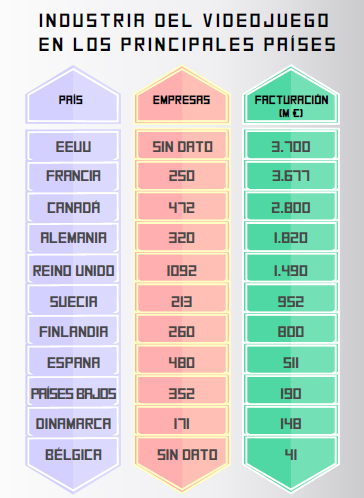
\includegraphics[width=0.6\textwidth]{images/estadodelarte/mercado/comparativa-internacional}
    \caption{Tabla extraída del Libro Blanco del videojuego (2016)}
\end{figure}

A pesar del estancamiento generalizado de la creación de empleo en el país, la industria del videojuego consiguió incrementar su plantilla un 32\% en el año 2015. En total hay 4.460 profesionales en la industria, entre empleados y colaboradores directos. Si incluimos las estimaciones de empleos que fueron generados de forma indirecta por la actividad de la industria, se alcanza un total de 7849 profesionales.

La comunidad autónoma con mayor peso en la industria es Cataluña, con el 38\% del empleo – sin duda, por la importante contribución de empresas como King y Social Point – y de la Comunidad de Madrid, con el 28\%. Juntas concentran el 66\% del empleo nacional. Le sigue Andalucía que representa un 10\% del total. Las sedes de los estudios de más envergadura y, por tanto, con mayor empleo están localizadas en estas comunidades. Según los datos recogidos, una característica relevante del empleo generado por el sector es su elevada tasa de estabilidad, dado que casi el 60\% de los contratos tiene carácter indefinido.

\subsection{Retos y tendencias actuales}
El videojuego ha sido y es una industria muy cambiante, que siempre ha intentado integrar las tecnologías más punteras, desde innovadores algoritmos de renderizado gráfico hasta exóticos dispositivos de interacción persona-ordenador.

A continuación, listaremos algunas de las tendencias que van a influir fuertemente en el mercado en los años venideros:

\subsubsection{eSports}
Los eSports, también llamados ``deportes electrónicos'', es el nombre por el cual se conocen las competiciones de videojuegos multijugador. En los eSports, los jugadores profesionales compiten entre ellos en diferentes categorías: disparos en primera persona, lucha, estrategia en tiempo real, MOBAs (Multiplayer Online Battle Arena)... La popularidad de este fenómeno ha llegado al punto en el que los principales torneos se celebran en grandes estadios, están retransmitidos en streaming por Internet e incluso están dotados con premios de grandes cantidades de dinero y que en ocasiones superan el millón de euros. Se trata de unos eventos de gran popularidad que cuentan enormes con perspectivas de crecimiento (a una tasa anual del 40\%). Esto ha provocado que se haya posicionado como un fenómeno de ocio estratégico.

\begin{figure}[h]
    \centering
    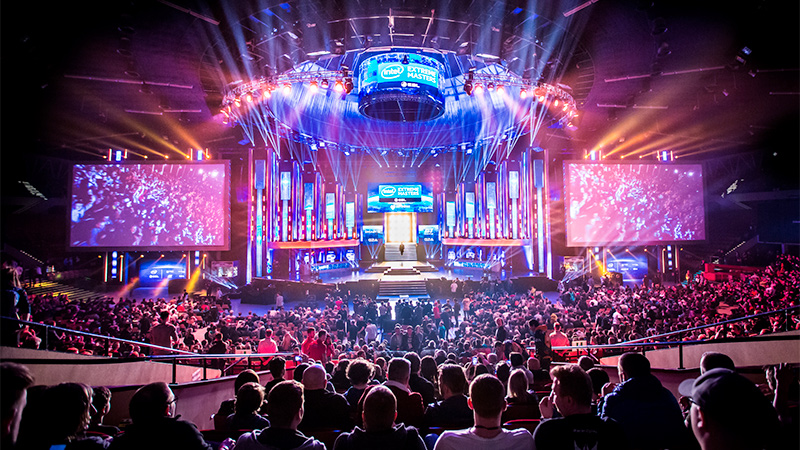
\includegraphics[width=0.8\textwidth]{images/estadodelarte/mercado/foto-torneo-esport}
    \caption{Fotografía del torneo Intel® Extreme Masters en Katowice, Polonia}
\end{figure}

El mercado de los eSports, generó en 2015 325 millones de dólares de ingresos, creciendo del 67\% con respecto al año anterior. Si la situación se mantiene, se espera que la cifra supere los mil millones de dólares en el año 2019, manteniendo un crecimiento anual superior al 40\%. En 2015, hubo 230 millones de personas que vieron partidos de competiciones de diversos deportes electrónicos, de los cuales 115 millones pueden ser clasificados como “entusiastas”, es decir, espectadores regulares y participantes no muy distintos de los que encontraríamos en los deportes convencionales. La plataforma de retransmisión en directo Twitch registro más de 800 millones de horas de contenidos de eSports en el periodo entre agosto de 2015 y mayo de 2016.

\begin{figure}[h]
    \centering
    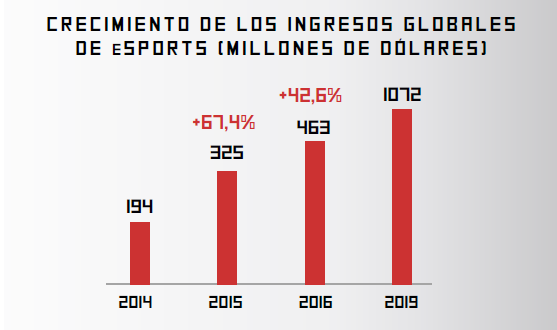
\includegraphics[width=0.8\textwidth]{images/estadodelarte/mercado/esport-crecimiento-ingreso}
    \caption{Tabla extraída del Libro Blanco del videojuego (2016)}
\end{figure}

Existen en España diferentes empresas que en la actualidad apuestan por el desarrollo de productos que aspiran a convertirse en eSports, es el caso de Digital Legends\footnote{http://www.digital-legends.com/}, Mercury Steam\footnote{https://www.mercurysteam.com/}, PixelCream Studio\footnote{http://pixelcreamstudio.com/}, Mechanical Boss\footnote{http://www.mechanicalboss.com/}, entre otros. Sin embargo, en la mayoría de las ocasiones un videojuego online se convierte en eSports de manera orgánica, basada en el reconocimiento que la comunidad online de jugadores activos de ese videojuego le otorga. Existen eso si casos en las que una gran marca apuesta porque su producto se convierta en un eSports, realizando grandes inversiones en base a una gran inversión en infraestructura, personal dedicado a la comunidad, servidores escalables para una gran masa de jugadores, premios para los torneos, entre otras muchas. 

Sin embargo, esta inversión no siempre esto asegura que su producto se convierta en un éxito. Para que un videojuego pueda convertirse en un eSport necesita contar con características básicas: tener un fuerte factor de competición, partidas cortas de no más de 1 hora, sin progresión in-game (la progresión debe basarse en las habilidades del jugador) atractivo sistema de espectador y tener un enfoque al 100\% internacional.

Pese a su gran dificultad, conseguir posicionar un producto como eSports, aporta una serie de beneficios y posibilidades: 
\begin{itemize}
\item Crear una base de fans, una comunidad, algo que aporta un núcleo de consumidores fieles al producto y que le da una nueva dimensión social, muy atractiva para muchos de los consumidores de videojuegos.
\item Prolongar la vida del producto; al ser competitivo, el jugador fija sus metas ante los otros jugadores, esto incentiva al usuario y le proporciona una motivación para seguir consumiendo.
\item Proporcionar mayor visibilidad, ya que, aunque los productos asentados son extremadamente sólidos, son muy reducidos, por lo cual hay una demanda latente de usuarios que buscan nuevos eSports.
\item Aumentar la fidelidad de los usuarios al tratarse de un mercado donde los usuarios tienen un índice de fidelidad mucho más alto que en otros.
\item Los jugadores, al estar involucrado con un producto competitivo, ven streaming, leen noticias, siguen torneos, participan en foros, lo que disminuye el riesgo de abandono del producto.
\end{itemize}

\begin{figure}[h]
    \centering
    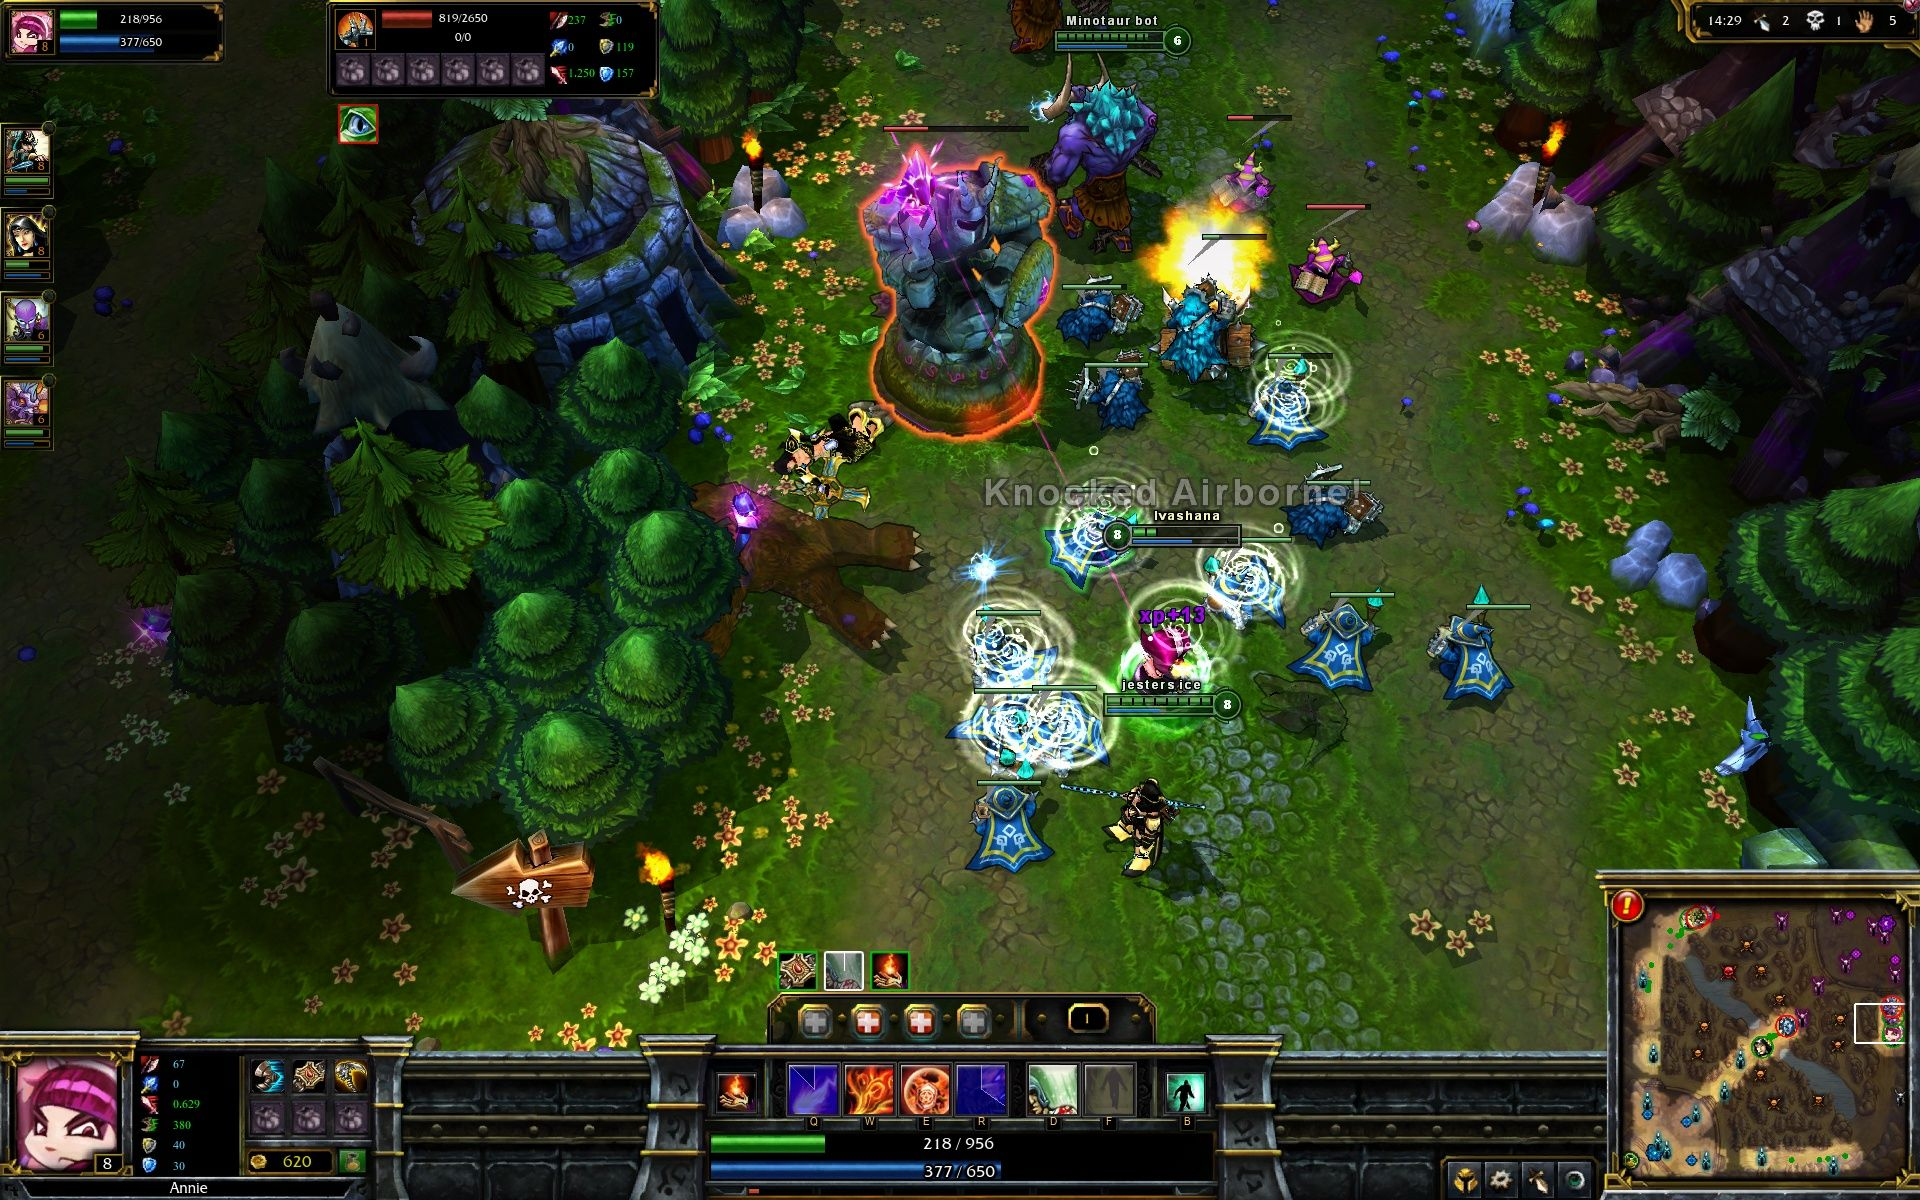
\includegraphics[width=0.8\textwidth]{images/estadodelarte/mercado/foto-lol}
    \caption{League of Legends, uno de los eSports más populares}
\end{figure}

Para una empresa pequeña, la producción de un eSports es, en principio inabarcable, inabarcable debido a la elevada inversión mencionada anteriormente. Sin embargo, la asociación con unos los partners correctos, ya establecidos en el sector, que pudieran invertir en el producto y le den visibilidad, puede dar una gran oportunidad a los pequeños desarrolladores que cuentan con una mayor flexibilidad con respecto a las grandes compañías, lo que les permite adaptarse más rápidamente a un mercado tan cambiante y mantener una relación directa con el feedback del usuario.

\subsubsection{Realidad Virtual y Realidad Aumentada}
La realidad virtual (normalmente abreviada como VR por las siglas inglesas de Virtual Reality) es la tecnología generada por sistemas informáticos que proporcionan un entorno audiovisual en 3D el que el usuario puede experimentar una inmersión total. Para ello, se hacen usos de cascos especiales equipados con pantallas y sensores de movimiento, los cuales normalmente se complementan con mandos equipados también con sensores para permitir una interacción más natural.
Por otro lado, la Realidad Aumentada o AR es una tecnología que superpone una capa de gráficos generados por ordenador sobre el entorno que rodea al jugador, con la que este puede interaccionar en tiempo real. A diferencia de la VR, no se requiere obligatoriamente de un hardware especial para poder implementar AR; basta únicamente de un dispositivo equipado con una pantalla y una cámara de vídeo, como podría ser un Smartphone.

\begin{figure}[h]
    \centering
    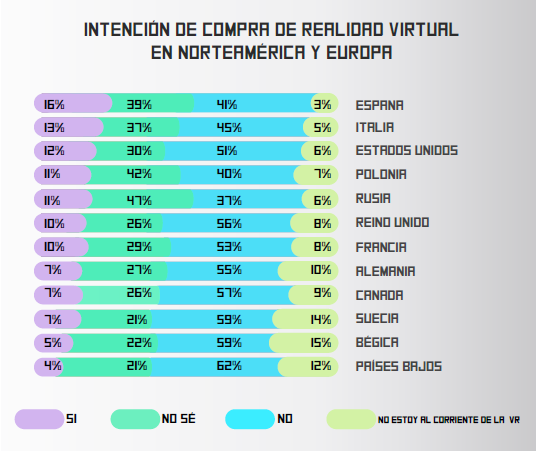
\includegraphics[width=0.8\textwidth]{images/estadodelarte/mercado/intencion-compra-vr}
    \caption{Tabla extraída del Libro Blanco del videojuego (2016)}
\end{figure}

Actualmente, existen varias propuestas de diversas compañías en lo que a equipo de VR se refiere. Vamos a mencionar algunas de las más importantes:
\begin{itemize}
\item \textbf{HTC Vive\footnote{https://www.vive.com/}}: es la propuesta de HTC y Valve, orientada a jugadores "hardcore" de PC. Disponible desde abril de 2016, el dispositivo requiere de un PC de gama alta (Valve recomienda un PC con una gráfica GeForce GTX 970). El kit de hardware incluye el casco equipado con dos pantallas de 1080x1200 puntos y 90Hz de frecuencia de actualización, dos sensores espaciales y dos mandos para registrar los movimientos de ambas manos, lo que crea le permite crear un entorno 100\% virtual en el que sumergir al jugador.

\item \textbf{OCULUS Rift\footnote{https://www.oculus.com/rift/}}: Es la propuesta más veterana de la lista. Empezó como un exitoso proyecto de Kickstarter en 2012 que más tarde fue adquirida por la empresa Facebook dos años más tarde. Al igual que HTC Vive, Oculus está formado por un casco equipado con pantallas de alta resolución, mandos con sensores de movimiento y dos sensores de posición. El equipo necesita estar conectado a un PC de alta gama para poder funcionar correctamente.

\item \textbf{Samsung Gear VR\footnote{http://www.samsung.com/es/wearables/gear-vr-sm-r325nzvaphe/}}: La propuesta de Samsung es mucho más sencilla y económica, orientado más a la reproducción de vídeo en 360º (concepto similar a la realidad virtual pero con interactividad limitada). El casco incluye una única pantalla y sus mandos carece de detección de movimiento. Estas limitaciones conllevan, por otro lado, un precio mucho más accesible que el de las otras alternativas (99€ contra los más de 500€ de las propuestas más completas)

\item \textbf{SONY PlayStation VR\footnote{https://www.playstation.com/explore/playstation-vr/}}: la propuesta de Sony fue lanzada en el año 2016. Al igual que otras alternativas, el sistema se basa en un casco equipado con dos pantallas y sensores de movimiento, pero su principal punto de venta es su compatibilidad con la consola PlayStation 4 de la misma marca. Esto permite aprovechar la potencia y los mandos de control de está de la consola.
\end{itemize}

\begin{figure}[!htb]
   \begin{minipage}{0.24\textwidth}
     \centering
     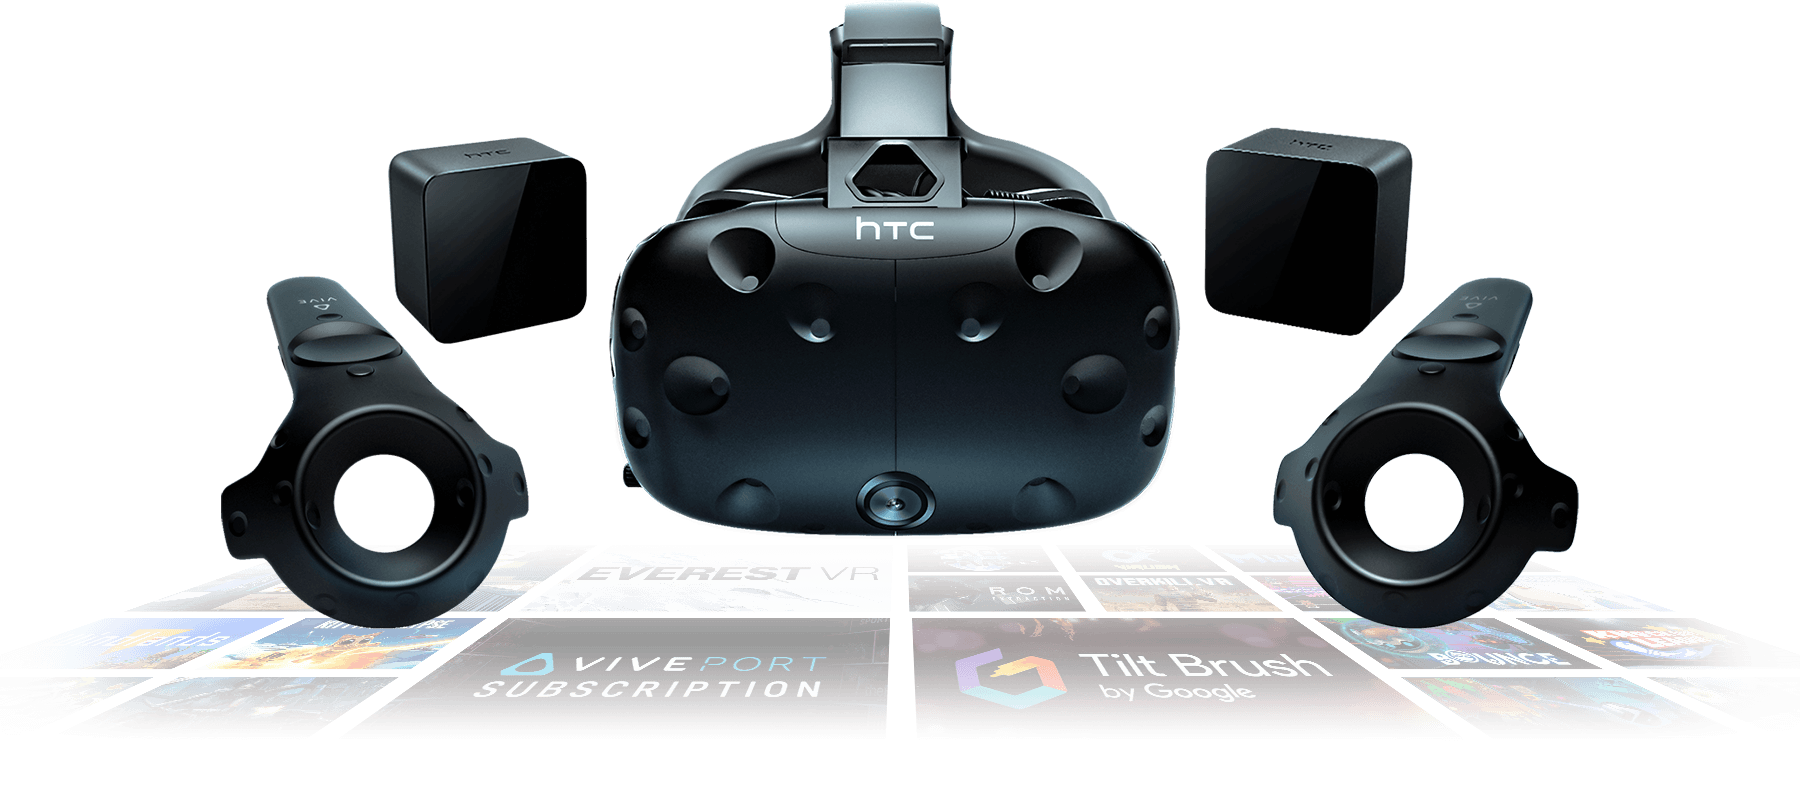
\includegraphics[width=0.7\linewidth, right]{images/estadodelarte/mercado/foto-htc-hive}
   \end{minipage}\hfill
   \begin {minipage}{0.24\textwidth}
     \centering
     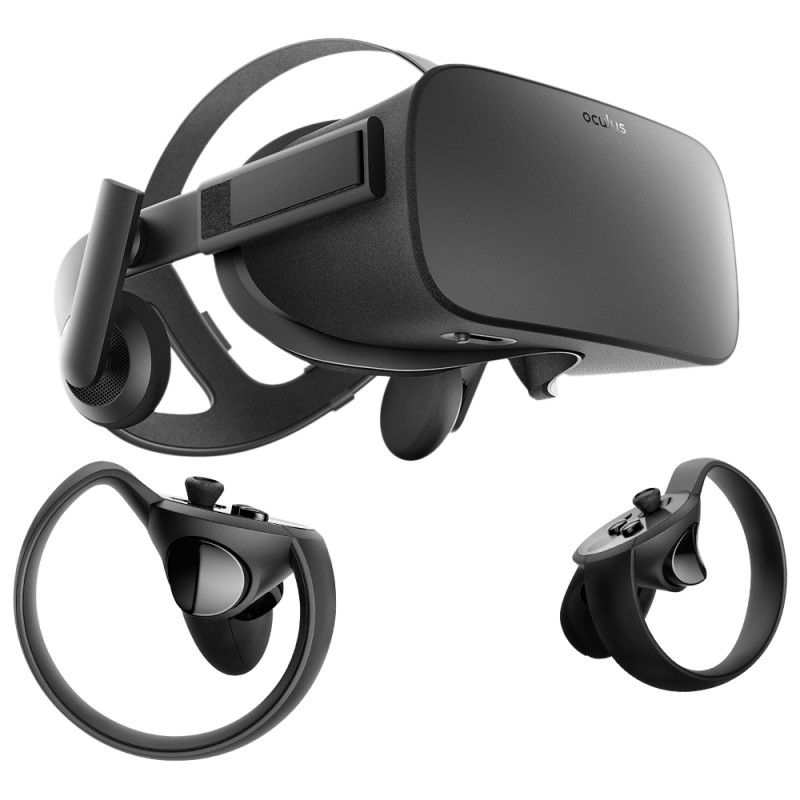
\includegraphics[width=0.7\linewidth, left]{images/estadodelarte/mercado/foto-oculus}
   \end{minipage}
      \begin {minipage}{0.24\textwidth}
     \centering
     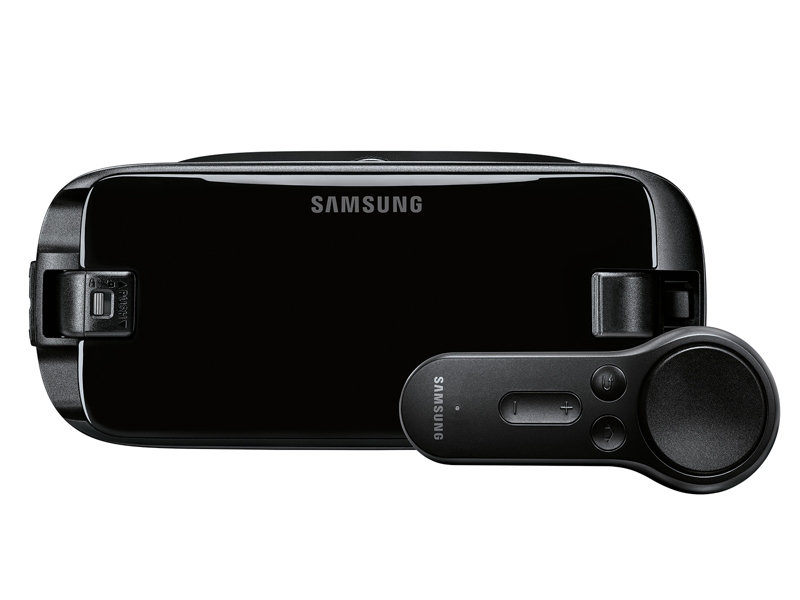
\includegraphics[width=0.7\linewidth, left]{images/estadodelarte/mercado/foto-samsung-vr}
   \end{minipage}
      \begin {minipage}{0.24\textwidth}
     \centering
     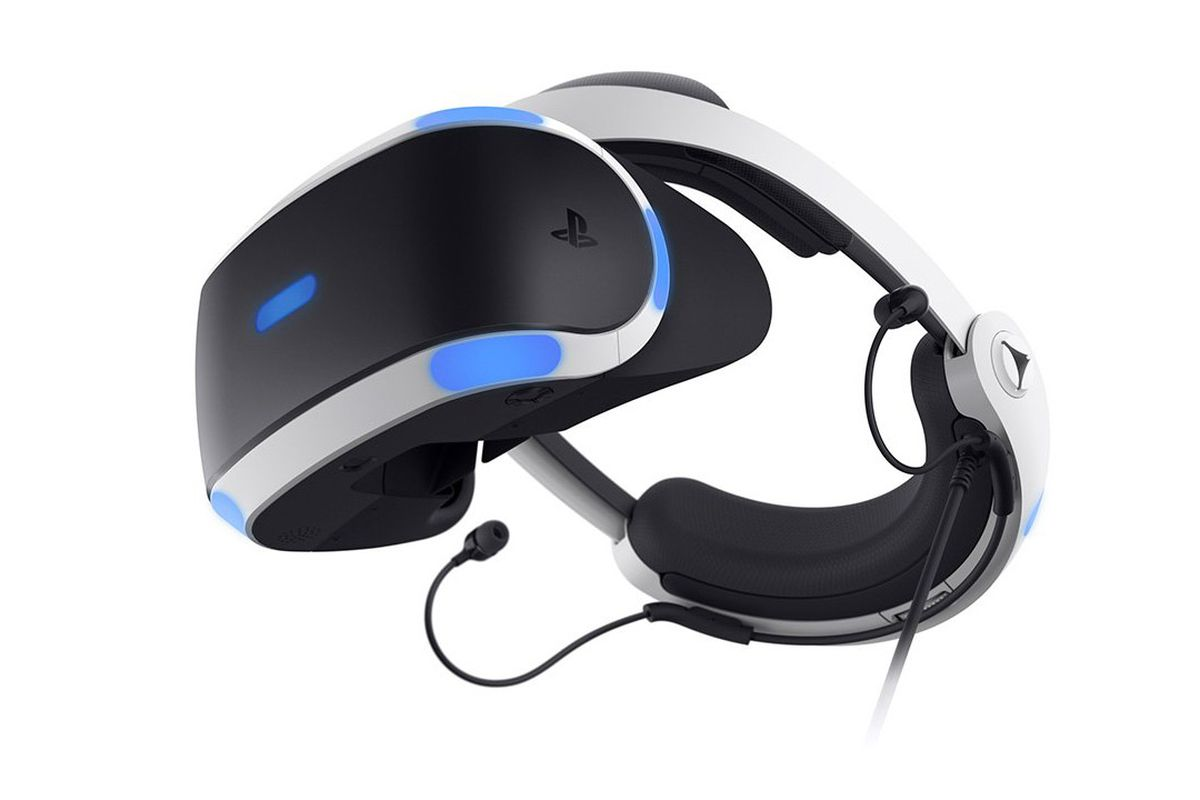
\includegraphics[width=0.7\linewidth, left]{images/estadodelarte/mercado/foto-sony-vr}
   \end{minipage}
   \caption{De izquierda a derecha HTC Vive, Oculus Rift, Samsung VR y PlayStation VR}
\end{figure}

\subsubsection{Web 4.0}
El termino Industria 4.0 fue acuñado por el Ministerio de Educación y Desarrollo alemán en su plan estratégico de 10 puntos del año 2016 para mejorar la educación, investigación e industria del país para adaptarlas a las tecnologías de Internet \cite{web_4_0}. La estrategia trata cinco áreas principales:
\begin{itemize}
\item Fuerte cooperación entre la investigación científica y las empresas.
\item Aumentar la innovación en el sector privado.
\item Diseminar las tecnologías punteras.
\item Internacionalizar la investigación y desarrollo.
\item Fondos para individuos con talento.
\end{itemize}

\begin{figure}[h]
    \centering
    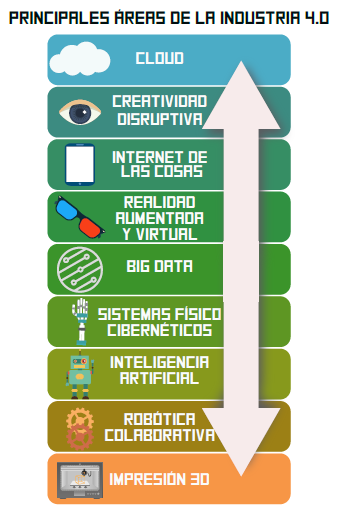
\includegraphics[width=0.6\textwidth]{images/estadodelarte/mercado/tabla-web-4}
    \caption{Tabla extraída del Libro Blanco del videojuego (2016)}
\end{figure}

De entre las distintas tecnologías que podrían categorizarse como parte de la industria 4.0, vamos a describir aquellas que tienen mayores aplicaciones en el desarrollo de videojuegos:

La computación en la nube, o Cloud Computing, es la tecnología que permite el acceso a servicios informáticos de forma rápida y sencilla a través de Internet. Aunque aún no se a podido implementar correctamente el Cloud Gaming (donde el juego es íntegramente ejecutado en la nueve, reduciendo la exigencia de potencia del sistema del jugador), si se utilizan sistemas en la nube en distintas áreas de los videojuegos. Especialmente notable es su uso para el control y almacenamiento de información en juegos multijugador en línea.

El Internet de las cosas es como se conoce a la tecnología que permite dotar de conexión a Internet a todo tipo de pequeños dispositivos como relojes, sistemas de domótica, drones, sensores de todo tipo, robots, etc. Esto permite implementar videojuegos en todo tipo de sistemas, desde consolas portátiles cada vez más pequeñas y económicas, pasando por juguetes interactivos y llegando a la posibilidad de gamificar con facilidad procesos industriales.

Big Data es el proceso de clasificar grandes volúmenes de datos para poder obtener relaciones interesantes y no evidentes entre ellos. El principal uso de las técnicas de BigData en la industria del Videojuego es el análisis de la información de los jugadores. Analizando datos de los jugadores tales como el género, la edad, la localización geográfica, los intereses, los gastos realizados, etc. es posible obtener estrategias de negocios eficientes.

Los sistemas Ciberfísicos son un nuevo tipo de sistemas con unos componentes hardware y software estrechamente interconectados, cada uno operando en su propio ámbito, operando e interaccionando de forma distinta dependiendo del contexto\cite{cyber_physics}. Entre sus aplicaciones se encuentran las redes eléctricas inteligentes, los sistemas de conducción automática de aviones y automóviles o la monitorización médica. Las interfaces de estos sistemas requieren de unas interfaces con un fuerte "lado humano" que permita un uso sencillo e intuitivo. Aquí se podrían utilizar los principios de diseño de juego que permitirían desarrollar un mejor puente entre el lado máquina y la parte de usuario.

La Impresión 3D, también conocida como la producción aditiva es una tecnología que permite producir objetos de forma más sencilla que con las técnicas anteriores. En combinación con las técnicas de escaneado 3D, los estudios de videojuego pueden generar de forma rápida y eficiente modelos 3D de todo tipo (personajes, mapas, objetos...).

\begin{figure}[h]
    \centering
    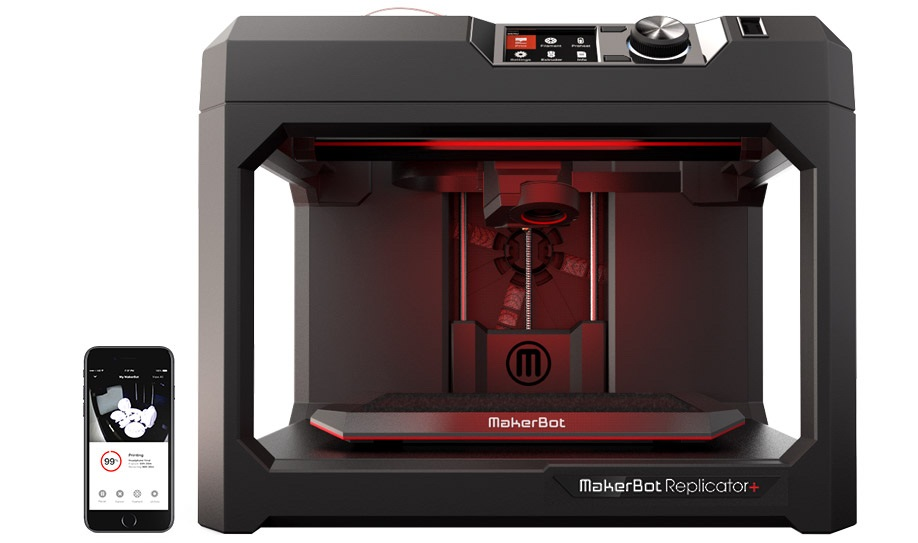
\includegraphics[width=0.8\textwidth]{images/estadodelarte/mercado/impresion-3d}
    \caption{Impresora 3d ``replicator'' de la compañía Makerbot}
\end{figure}

Las nuevas tecnologías de la industria 4.0 serán de gran ayuda para el desarrollo de videojuego. Pero es posible que la industria 4.0 también ofrezca valor a la industria 4.0 en su conjunto. Dado que la creación de videojuegos es una actividad industrial que está vinculada a diferentes áreas de conocimiento que trabajan juntas para conseguir ofrecer un producto, las técnicas y paradigmas utilizados tienen mucho en común con la nueva forma de trabajar de la industria 4.0, por lo que es posible que puedan extrapolarse a otras industrias, permitiendo una mejor adaptación a los cambios.
